\documentclass{srmreport}
\title{Major Project Report}
\author{Supratik Chatterjee (RA1511003040196)}
% \second{Sanjeev Siva (RA1511003040193)}
% \third{Shubham Bagdiya (RA1511003040258)}
\topic{Project NASTY}
\obj{Major Project Report}
\desc{news aggregation and summarization}
\dept{Computer Science Engineering}
\bonafide{Supratik Chatterjee (RA1511003040196)}
\date{APRIL 2019}
\thanks{
I place my gratitude with our respected chancellor of SRM Institute of Science and Technology, to have provided the required infrastructure, to hone my skills. I also thank my teachers for their guidance and teachings, without which I would not be able to learn what I know as efficiently as I do.\\\\We extend this opportunity to extend our heartfelt gratitude to our respected Dean {\bfseries Dr. K. Duraivelu} for his impeccable guidance.\\\\We deeply express our sincere thanks  to our Head of Department  {\bfseries Dr. S. Prasanna Devi}, for encouraging and allowing us to present the project on the topic, {\bfseries News Analysis and Summarization Tool}, at our department  premises  for the partial  fulfillment  of the requirements leading to the award of B-Tech degree.\\\\It is our privilege to express our sincerest regards to our project coordinator, {\bfseries Mr. Muthurasu N.} for his valuable inputs, able guidance, encouragement, whole-hearted cooperation and constructive criticism throughout the duration of our project.\\\\We take this opportunity to thank all our faculty members and management who have directly or indirectly helped our project. Last but not the least we express our thanks to our friends for their cooperation and support.
}
\guide{
Mr. N. Muthurasu\\
B.E., M.Tech,\\\\
Assistant Professor\\
Department of CSE\\
SRM IST\\
Vadapalani,Chennai-600026\\\\
}
\hod{
Dr. S. Prasanna Devi\\
B.E., M.Tech, Ph.D.,\\
PGDHRM, PDF(IISc),\\
Head of the Department\\
Department of CSE\\
SRM IST\\
Vadapalani,Chennai-600026\\
}
%\bonafide{%\begin{doublespacing}}
\abstract{
In the modern day field of media, news is majorly affected by the social platforms such as Facebook, Twitter, etc. It becomes necessary to understand all the facts of an event, and to quantify, or relate them to understand it. Most humans do not have the dedication or time to study all the events at all the time, as time is always limited. However, an aggregation and analysis system on a computer could do it for them. A computer can form links and store endless amounts of data which would only be affected by the amount of storage space available and the storage algorithm being made use of. Apart from that advantage we have the advantage of having programs such as Hadoop and MongoDB to take care of a lot of work for us. This project has been worked upon with an idea in mind, to create a common platform for people to fetch aggregated data from multiple news agencies through an abstraction.
}
\begin{document}
\maketitle
\setlength{\columnsep}{10pt}
\chapter{Introduction}
When dealing with news papers, it becomes a tedious chore to understand which one to follow and why. A lot of times, we see that in order for people to report an event, they sometimes have to withhold some little pieces only to reveal those at a later date. Apart from these, there is also the part where  they need to be stored categorically to create a record of the modern history which keeps growing more and more opaque due to the complications everyday. So, how do we keep track of all facts while making sure we understand all related facets to an event?
\par The solution is by relying on autonomous systems to work towards continuous content fetching, analyzing, aggregating and relating facts. But where can a person find the facts? It so happens that most major news channels offer a format known as RSS, to fetch the data. However, it is nigh impossible for us to keep track with the humongous number of news networks that exist within our country alone (the number being 1,05,443, of which, 13,661 are English Newspapers), let alone that of news channels all over the world. So in order to reduce the generation of noisy data, we reduce the scope to work with the most prominents ones.
\par The prominent news channels provide a certain utility known as an Atom feed, or RSS feed. These feeds have been shown in this section. 
\begin{figure}[h]
\center
\begin{multicols}{2}
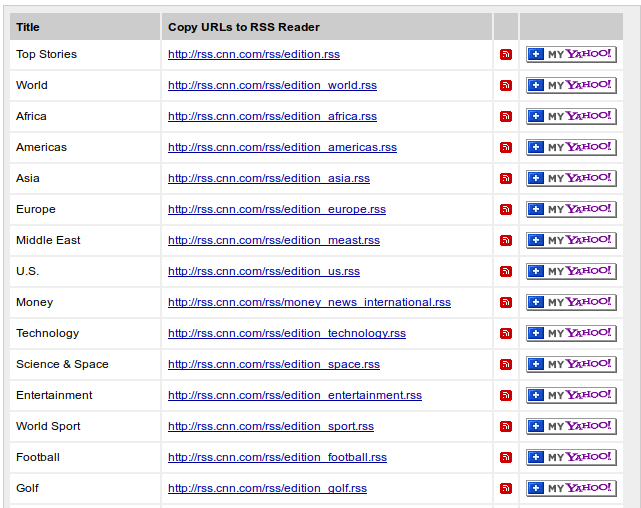
\includegraphics[scale=0.3]{res/rssfeeds/cnnlistings}\\
\caption{CNN RSS Listings}\vspace{0.5em}
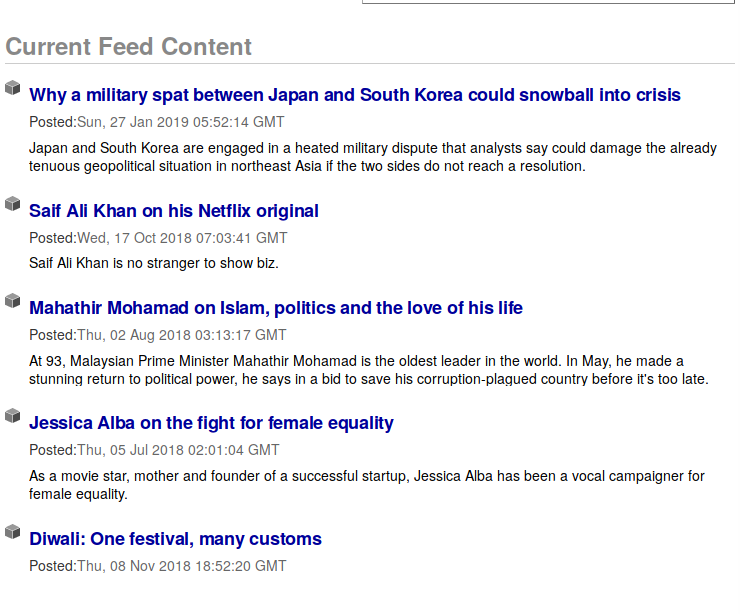
\includegraphics[scale=0.3]{res/rssfeeds/cnnrss}\\
\caption{CNN RSS feed}
\end{multicols}
\begin{multicols}{2}
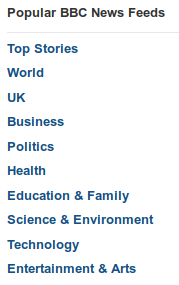
\includegraphics[scale=0.6]{res/rssfeeds/bbclistings}\\
\caption{BBC RSS Listings}\vspace{0.5em}
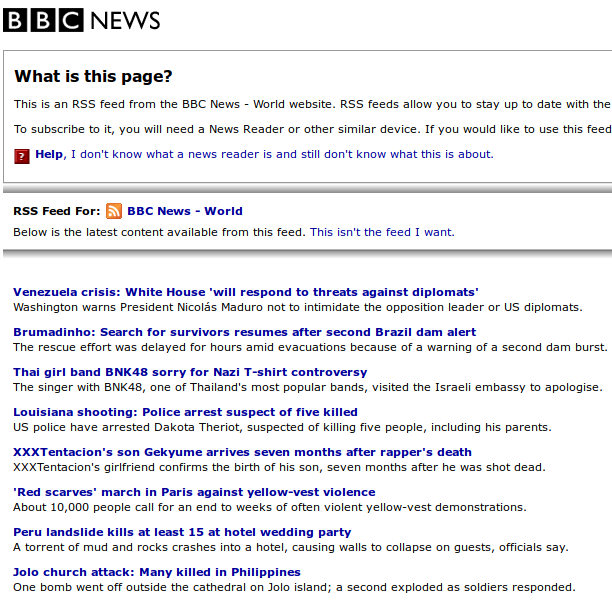
\includegraphics[scale=0.3]{res/rssfeeds/bbcrss}\\
\caption{BBC RSS feed}
\end{multicols}
\end{figure}
These utilities are however under-utilized in most cases. Our work is to exploit this resource, made available from news networks, and manage it to maximize their usage.

\chapter{Project Work}

Facts collection, aggregation and relation is everything this project is about. RSS feeds usually contain the shortened form of all the events, covering only the facts of the event.

\section{The Concept}
News articles contain well structured sentences that contain information in a human-readable language using the least amount of complicated words as can be managed. 
\par To obtain the content, we make use of a Focused Incremental Web Crawler(A web crawler that extracts only specific content at a relatively shallow depth). This content is brought and stored for consideration in a pre-determined storage unit. This then moves on for analysis.
\par Facts aggregation is a lot about analysis of the text in the content, to find for three primary things, which are attributes, relations and involvement in events. These three are the specific information required. This involves the usage of NLP methodologies such as Named Entity Relations, Parts of Speech Tagging, Anaphora Resolution, and several others, which are to work together to reduce the amount of useless data to be stored about entities.

% Focused Incremental Web Crawler-Centralisation-Web Scraping-Facts Aggregation through NLP-Summarization-Storage-Relational Heaps over NoSQL-RSS-More concepts.

\section{Problem Statement}
Aggregation and analysis of news over network, from several channels to remove repetitions and increase efficient centralization of factual data of any event, location or an object.

\section{Proposed Solution}
The solution is to make use of an observer program to do it all, at regular intervals by utilizing a programming language, which in this particular case, for prototyping, would be through python.

\section{Obstacles}
There are three obstacles to this:
\subsection{Relation Extraction}
\subsection{Reference Resolution}
\subsection{Metadata Repository}

\section{Advantages}

\section{Future Scope}


\section{Available tools}
There are absolutely no tools available of this kind. There are several that forward the RSS feeds onto devices. But none that analyze to obtain all facts and aggregate it at a single point. A few of the more remarkable ones are specified here for your consideration.

\subsection{News API}


\section{Tools Studied and Used}
\subsection{Python 3}
\subsection{nltk}
\subsection{Stanford CoreNLP}
\subsection{RSS}
\subsection{JSON}
\subsection{MongoDB}

\section{Theories}

\chapter{Conclusion}
\bibliographystyle{plain}
\bibliography{refer}
\end{document}
